\documentclass[border=4pt]{standalone}
\usepackage[T1]{fontenc}
\usepackage{lmodern}
\usepackage{amsmath,amssymb}
\usepackage{tikz}
\usetikzlibrary{positioning,calc}
\usepackage{pgfplots}
\usepgfplotslibrary{statistics}
\pgfplotsset{compat=1.18}

%% ── Colours (identical to draw_figure2*.py) ─────────────────────────────────
\definecolor{myblue}  {RGB}{55, 119, 189}
\definecolor{myred}   {RGB}{210,  70,  70}
\definecolor{mygreen} {RGB}{ 50, 155,  70}
\definecolor{myorange}{RGB}{230, 130,  40}
\definecolor{mygray}  {RGB}{130, 130, 130}

\begin{document}
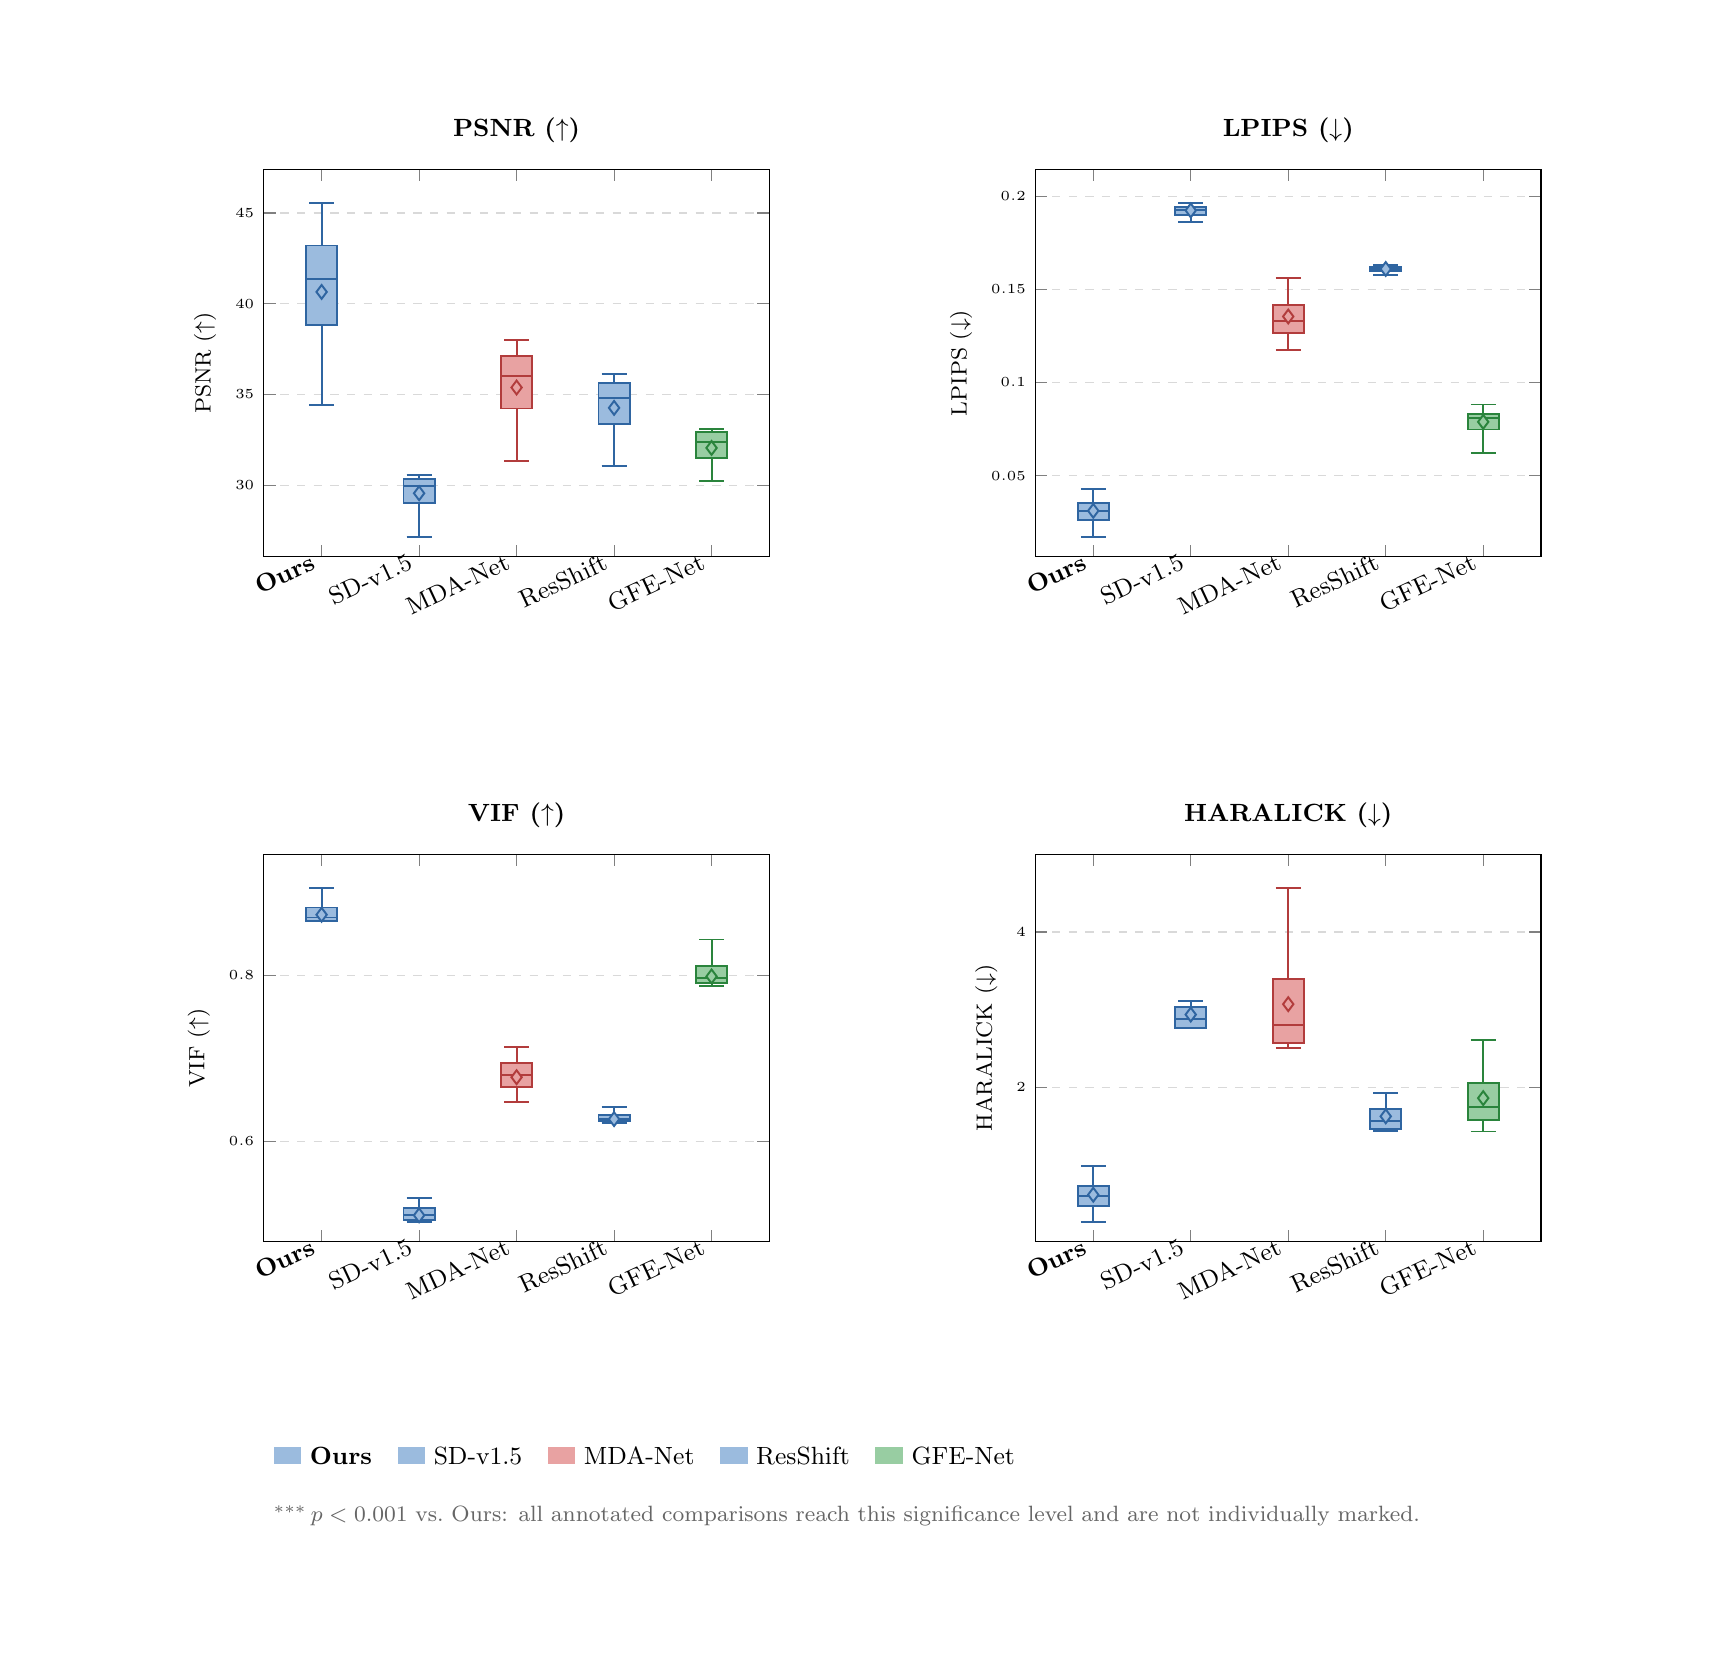
\begin{tikzpicture}[font=\small]
\useasboundingbox (-3.0cm,1.8cm) rectangle (18.3cm,-18.7cm);

% ── PSNR (row=0, col=0) ─────────────────────────────
\begin{axis}[
  name=ax00,
  at={(0.00cm,0.00cm)},
  anchor=north west,
  width=8.0cm,
  height=6.5cm,
  boxplot/draw direction=y,
  boxplot/box extend=0.32,
  xtick={1,...,5},
  xticklabels={{\textbf{Ours}},{SD-v1.5},{MDA-Net},{ResShift},{GFE-Net}},
  xticklabel style={rotate=25, anchor=east, font=\small},
  ymin=26.0535, ymax=47.4010,
  ylabel={PSNR ($\uparrow$)},
  ylabel style={font=\footnotesize},
  ymajorgrids=true,
  grid style={dashed, gray!30},
  tick style={thin},
  every tick label/.style={font=\footnotesize},
  clip=false,
  scaled y ticks=false,
  y tick label style={font=\tiny, /pgf/number format/fixed, /pgf/number format/precision=3},
  title={PSNR ($\uparrow$)},
  title style={font=\small\bfseries},
]

% Ours
\addplot[
  boxplot prepared={
    lower whisker=34.3978,
    lower quartile=38.8105,
    median=41.3518,
    upper quartile=43.2069,
    upper whisker=45.5607,
    average=40.6481,
  },
  fill=myblue!50, draw=myblue!85!black, line width=0.7pt,
  boxplot/every average/.style={mark=diamond*, mark size=2.5pt, fill=myblue, draw=myblue!70!black},
] coordinates {};
% SD-v1.5
\addplot[
  boxplot prepared={
    lower whisker=27.1577,
    lower quartile=29.0205,
    median=29.9402,
    upper quartile=30.3244,
    upper whisker=30.5805,
    average=29.5489,
  },
  fill=myblue!50, draw=myblue!85!black, line width=0.7pt,
  boxplot/every average/.style={mark=diamond*, mark size=2.5pt, fill=myblue, draw=myblue!70!black},
] coordinates {};
% MDA-Net
\addplot[
  boxplot prepared={
    lower whisker=31.3439,
    lower quartile=34.2220,
    median=36.0057,
    upper quartile=37.1273,
    upper whisker=38.0191,
    average=35.3790,
  },
  fill=myred!50, draw=myred!85!black, line width=0.7pt,
  boxplot/every average/.style={mark=diamond*, mark size=2.5pt, fill=myred, draw=myred!70!black},
] coordinates {};
% ResShift
\addplot[
  boxplot prepared={
    lower whisker=31.0604,
    lower quartile=33.3783,
    median=34.8043,
    upper quartile=35.6180,
    upper whisker=36.0989,
    average=34.2565,
  },
  fill=myblue!50, draw=myblue!85!black, line width=0.7pt,
  boxplot/every average/.style={mark=diamond*, mark size=2.5pt, fill=myblue, draw=myblue!70!black},
] coordinates {};
% GFE-Net
\addplot[
  boxplot prepared={
    lower whisker=30.2316,
    lower quartile=31.5165,
    median=32.3927,
    upper quartile=32.9082,
    upper whisker=33.1113,
    average=32.0483,
  },
  fill=mygreen!50, draw=mygreen!85!black, line width=0.7pt,
  boxplot/every average/.style={mark=diamond*, mark size=2.5pt, fill=mygreen, draw=mygreen!70!black},
] coordinates {};

\end{axis}

% ── LPIPS (row=0, col=1) ─────────────────────────────
\begin{axis}[
  name=ax01,
  at={(9.80cm,0.00cm)},
  anchor=north west,
  width=8.0cm,
  height=6.5cm,
  boxplot/draw direction=y,
  boxplot/box extend=0.32,
  xtick={1,...,5},
  xticklabels={{\textbf{Ours}},{SD-v1.5},{MDA-Net},{ResShift},{GFE-Net}},
  xticklabel style={rotate=25, anchor=east, font=\small},
  ymin=0.0066, ymax=0.2143,
  ylabel={LPIPS ($\downarrow$)},
  ylabel style={font=\footnotesize},
  ymajorgrids=true,
  grid style={dashed, gray!30},
  tick style={thin},
  every tick label/.style={font=\footnotesize},
  clip=false,
  scaled y ticks=false,
  y tick label style={font=\tiny, /pgf/number format/fixed, /pgf/number format/precision=3},
  title={LPIPS ($\downarrow$)},
  title style={font=\small\bfseries},
]

% Ours
\addplot[
  boxplot prepared={
    lower whisker=0.0173,
    lower quartile=0.0264,
    median=0.0311,
    upper quartile=0.0353,
    upper whisker=0.0427,
    average=0.0312,
  },
  fill=myblue!50, draw=myblue!85!black, line width=0.7pt,
  boxplot/every average/.style={mark=diamond*, mark size=2.5pt, fill=myblue, draw=myblue!70!black},
] coordinates {};
% SD-v1.5
\addplot[
  boxplot prepared={
    lower whisker=0.1860,
    lower quartile=0.1898,
    median=0.1923,
    upper quartile=0.1942,
    upper whisker=0.1964,
    average=0.1923,
  },
  fill=myblue!50, draw=myblue!85!black, line width=0.7pt,
  boxplot/every average/.style={mark=diamond*, mark size=2.5pt, fill=myblue, draw=myblue!70!black},
] coordinates {};
% MDA-Net
\addplot[
  boxplot prepared={
    lower whisker=0.1176,
    lower quartile=0.1264,
    median=0.1332,
    upper quartile=0.1418,
    upper whisker=0.1562,
    average=0.1354,
  },
  fill=myred!50, draw=myred!85!black, line width=0.7pt,
  boxplot/every average/.style={mark=diamond*, mark size=2.5pt, fill=myred, draw=myred!70!black},
] coordinates {};
% ResShift
\addplot[
  boxplot prepared={
    lower whisker=0.1576,
    lower quartile=0.1598,
    median=0.1610,
    upper quartile=0.1618,
    upper whisker=0.1631,
    average=0.1609,
  },
  fill=myblue!50, draw=myblue!85!black, line width=0.7pt,
  boxplot/every average/.style={mark=diamond*, mark size=2.5pt, fill=myblue, draw=myblue!70!black},
] coordinates {};
% GFE-Net
\addplot[
  boxplot prepared={
    lower whisker=0.0620,
    lower quartile=0.0748,
    median=0.0809,
    upper quartile=0.0833,
    upper whisker=0.0882,
    average=0.0789,
  },
  fill=mygreen!50, draw=mygreen!85!black, line width=0.7pt,
  boxplot/every average/.style={mark=diamond*, mark size=2.5pt, fill=mygreen, draw=mygreen!70!black},
] coordinates {};

\end{axis}

% ── VIF (row=1, col=0) ─────────────────────────────
\begin{axis}[
  name=ax10,
  at={(0.00cm,-8.70cm)},
  anchor=north west,
  width=8.0cm,
  height=6.5cm,
  boxplot/draw direction=y,
  boxplot/box extend=0.32,
  xtick={1,...,5},
  xticklabels={{\textbf{Ours}},{SD-v1.5},{MDA-Net},{ResShift},{GFE-Net}},
  xticklabel style={rotate=25, anchor=east, font=\small},
  ymin=0.4790, ymax=0.9460,
  ylabel={VIF ($\uparrow$)},
  ylabel style={font=\footnotesize},
  ymajorgrids=true,
  grid style={dashed, gray!30},
  tick style={thin},
  every tick label/.style={font=\footnotesize},
  clip=false,
  scaled y ticks=false,
  y tick label style={font=\tiny, /pgf/number format/fixed, /pgf/number format/precision=3},
  title={VIF ($\uparrow$)},
  title style={font=\small\bfseries},
]

% Ours
\addplot[
  boxplot prepared={
    lower whisker=0.8657,
    lower quartile=0.8661,
    median=0.8700,
    upper quartile=0.8820,
    upper whisker=0.9058,
    average=0.8733,
  },
  fill=myblue!50, draw=myblue!85!black, line width=0.7pt,
  boxplot/every average/.style={mark=diamond*, mark size=2.5pt, fill=myblue, draw=myblue!70!black},
] coordinates {};
% SD-v1.5
\addplot[
  boxplot prepared={
    lower whisker=0.5032,
    lower quartile=0.5047,
    median=0.5107,
    upper quartile=0.5200,
    upper whisker=0.5315,
    average=0.5109,
  },
  fill=myblue!50, draw=myblue!85!black, line width=0.7pt,
  boxplot/every average/.style={mark=diamond*, mark size=2.5pt, fill=myblue, draw=myblue!70!black},
] coordinates {};
% MDA-Net
\addplot[
  boxplot prepared={
    lower whisker=0.6476,
    lower quartile=0.6653,
    median=0.6798,
    upper quartile=0.6946,
    upper whisker=0.7134,
    average=0.6774,
  },
  fill=myred!50, draw=myred!85!black, line width=0.7pt,
  boxplot/every average/.style={mark=diamond*, mark size=2.5pt, fill=myred, draw=myred!70!black},
] coordinates {};
% ResShift
\addplot[
  boxplot prepared={
    lower whisker=0.6223,
    lower quartile=0.6251,
    median=0.6271,
    upper quartile=0.6316,
    upper whisker=0.6414,
    average=0.6268,
  },
  fill=myblue!50, draw=myblue!85!black, line width=0.7pt,
  boxplot/every average/.style={mark=diamond*, mark size=2.5pt, fill=myblue, draw=myblue!70!black},
] coordinates {};
% GFE-Net
\addplot[
  boxplot prepared={
    lower whisker=0.7870,
    lower quartile=0.7910,
    median=0.7966,
    upper quartile=0.8119,
    upper whisker=0.8434,
    average=0.7989,
  },
  fill=mygreen!50, draw=mygreen!85!black, line width=0.7pt,
  boxplot/every average/.style={mark=diamond*, mark size=2.5pt, fill=mygreen, draw=mygreen!70!black},
] coordinates {};

\end{axis}

% ── HARALICK (row=1, col=1) ─────────────────────────────
\begin{axis}[
  name=ax11,
  at={(9.80cm,-8.70cm)},
  anchor=north west,
  width=8.0cm,
  height=6.5cm,
  boxplot/draw direction=y,
  boxplot/box extend=0.32,
  xtick={1,...,5},
  xticklabels={{\textbf{Ours}},{SD-v1.5},{MDA-Net},{ResShift},{GFE-Net}},
  xticklabel style={rotate=25, anchor=east, font=\small},
  ymin=0.0172, ymax=4.9971,
  ylabel={HARALICK ($\downarrow$)},
  ylabel style={font=\footnotesize},
  ymajorgrids=true,
  grid style={dashed, gray!30},
  tick style={thin},
  every tick label/.style={font=\footnotesize},
  clip=false,
  scaled y ticks=false,
  y tick label style={font=\tiny, /pgf/number format/fixed, /pgf/number format/precision=3},
  title={HARALICK ($\downarrow$)},
  title style={font=\small\bfseries},
]

% Ours
\addplot[
  boxplot prepared={
    lower whisker=0.2748,
    lower quartile=0.4823,
    median=0.5997,
    upper quartile=0.7324,
    upper whisker=0.9859,
    average=0.6216,
  },
  fill=myblue!50, draw=myblue!85!black, line width=0.7pt,
  boxplot/every average/.style={mark=diamond*, mark size=2.5pt, fill=myblue, draw=myblue!70!black},
] coordinates {};
% SD-v1.5
\addplot[
  boxplot prepared={
    lower whisker=2.7602,
    lower quartile=2.7675,
    median=2.8853,
    upper quartile=3.0301,
    upper whisker=3.1183,
    average=2.9381,
  },
  fill=myblue!50, draw=myblue!85!black, line width=0.7pt,
  boxplot/every average/.style={mark=diamond*, mark size=2.5pt, fill=myblue, draw=myblue!70!black},
] coordinates {};
% MDA-Net
\addplot[
  boxplot prepared={
    lower whisker=2.5120,
    lower quartile=2.5704,
    median=2.7991,
    upper quartile=3.3981,
    upper whisker=4.5678,
    average=3.0719,
  },
  fill=myred!50, draw=myred!85!black, line width=0.7pt,
  boxplot/every average/.style={mark=diamond*, mark size=2.5pt, fill=myred, draw=myred!70!black},
] coordinates {};
% ResShift
\addplot[
  boxplot prepared={
    lower whisker=1.4380,
    lower quartile=1.4644,
    median=1.5676,
    upper quartile=1.7277,
    upper whisker=1.9244,
    average=1.6298,
  },
  fill=myblue!50, draw=myblue!85!black, line width=0.7pt,
  boxplot/every average/.style={mark=diamond*, mark size=2.5pt, fill=myblue, draw=myblue!70!black},
] coordinates {};
% GFE-Net
\addplot[
  boxplot prepared={
    lower whisker=1.4350,
    lower quartile=1.5799,
    median=1.7499,
    upper quartile=2.0568,
    upper whisker=2.6122,
    average=1.8639,
  },
  fill=mygreen!50, draw=mygreen!85!black, line width=0.7pt,
  boxplot/every average/.style={mark=diamond*, mark size=2.5pt, fill=mygreen, draw=mygreen!70!black},
] coordinates {};

\end{axis}

\node[anchor=north west, font=\small] at (0cm,-16.10cm) {
  \tikz{\fill[myblue!50] (0,0) rectangle (0.35cm,0.22cm);}~\textbf{Ours}\quad \tikz{\fill[myblue!50] (0,0) rectangle (0.35cm,0.22cm);}~SD-v1.5\quad \tikz{\fill[myred!50] (0,0) rectangle (0.35cm,0.22cm);}~MDA-Net\quad \tikz{\fill[myblue!50] (0,0) rectangle (0.35cm,0.22cm);}~ResShift\quad \tikz{\fill[mygreen!50] (0,0) rectangle (0.35cm,0.22cm);}~GFE-Net
};

\node[anchor=north west, font=\footnotesize, text=gray!80!black] at (0cm,-16.85cm) {
  $^{***}$\,$p<0.001$ vs.\ Ours: all annotated comparisons reach this significance level and are not individually marked.
};

\end{tikzpicture}

\end{document}